\documentclass[12pt,a4paper]{article}

\usepackage[utf8]{inputenc}
\usepackage[T1]{fontenc}
\usepackage[english]{babel}
\usepackage{lmodern}
\usepackage[margin=2.6cm]{geometry}
\usepackage{amsmath,amssymb}
\usepackage{booktabs}
\usepackage{graphicx}
\usepackage{float}
\usepackage{listings}
\usepackage{xcolor}
\usepackage[hidelinks]{hyperref}

\graphicspath{{../figures/}}

\lstset{basicstyle=\ttfamily\small, frame=single, breaklines=true,
        columns=fullflexible, backgroundcolor=\color{gray!8}}

\newcommand{\act}[1]{\texttt{#1}}

\title{Process Mining and Formal Verification of the\\
       Volvo IT Incident Management Process\\
       \large BPI Challenge 2013}
\author{Formal Methods}
\date{\today}

\begin{document}
\maketitle

\begin{abstract}
This report analyses the BPI Challenge 2013 event logs from Volvo IT Belgium's
VINST incident and problem management system. Three discovery algorithms are
compared, model quality is assessed on four conformance dimensions, and eight
temporal properties are verified against every case using finite-trace linear
temporal logic. Three findings emerge. Rework dominates the process: fewer than
half of all recorded events are the first occurrence of their activity within a
case. The documented procedure of queueing an incident before working it is
violated in the large majority of cases, a deviation established by formal
verification rather than by inspection. And the Alpha miner fails on this log in
a way that is predicted by theory rather than caused by defect, because almost
every case contains a length-one loop that the algorithm cannot represent.
\end{abstract}

\tableofcontents
\newpage

\section{Introduction}

\subsection{Context}

Process mining derives models of real processes from the event logs that
information systems record as a by-product of their operation. Where a
conventional process model states how work is supposed to proceed, a discovered
model states how it actually proceeded. The gap between the two is the object of
study.

This report applies process discovery, conformance checking and formal
verification to the BPI Challenge 2013 dataset: the incident and problem
management logs of Volvo IT Belgium, recorded by the VINST service management
system. The dataset is a standard benchmark, which makes the results here
comparable with published work.

\subsection{Objectives}

\begin{enumerate}
  \item Derive process models from the logs and compare three discovery
        algorithms on four measures of model quality.
  \item Specify properties of the incident process in temporal logic and verify
        them against every recorded case.
  \item Quantify where time is spent and identify the structural sources of
        delay.
  \item Determine whether the process as executed matches the process as
        documented.
\end{enumerate}

\subsection{Structure}

Section~\ref{sec:foundations} sets out the formal apparatus. Section~\ref{sec:dataset}
describes the logs and the one modelling decision the dataset forces.
Section~\ref{sec:discovery} compares the discovery algorithms;
Section~\ref{sec:performance} analyses time; Section~\ref{sec:verification}
presents the formal verification. Section~\ref{sec:health} aggregates the
measures, Section~\ref{sec:architecture} describes the implementation, and
Section~\ref{sec:conclusions} states the conclusions and the limits of the
analysis.

\section{Theoretical foundations}\label{sec:foundations}

\subsection{Event logs}

An event log is a multiset of traces. A trace is a finite sequence of events
belonging to one case, ordered by timestamp. Each event carries at minimum a
case identifier, an activity name and a timestamp; the logs analysed here carry
further attributes recording the organisation and resource involved.

Writing $\Sigma$ for the set of activities, a trace is an element of $\Sigma^*$
and a log is a multiset over $\Sigma^*$. Two traces with the same activity
sequence belong to the same \emph{variant}. The number of distinct variants
relative to the number of cases measures how standardised a process is.

\subsection{Petri nets}

A Petri net is a tuple $N = (P, T, F)$ where $P$ and $T$ are disjoint finite
sets of places and transitions and $F \subseteq (P \times T) \cup (T \times P)$
is the flow relation. A marking assigns tokens to places; a transition is
enabled when each of its input places holds a token, and firing it consumes
those tokens and produces one in each output place. A labelled net maps
transitions to activities, with unlabelled (silent) transitions permitted to
express routing that corresponds to no recorded event.

An accepting Petri net additionally fixes an initial and a final marking. A
trace is \emph{replayable} if some firing sequence whose visible labels spell
the trace leads from the initial to the final marking.

\subsection{Conformance dimensions}

Model quality is not a single quantity. Four dimensions are standard, and they
trade off against one another, so all four must be reported together.

\begin{description}
  \item[Fitness] The extent to which the model can replay the traces in the log.
        A fitness of $1$ means every observed case is replayable. Low fitness
        means the model forbids behaviour that actually occurred.
  \item[Precision] The converse: the extent to which the model forbids behaviour
        that never occurred. Low precision indicates an over-permissive model,
        in the limit a ``flower'' model that permits any sequence whatsoever and
        therefore fits perfectly while explaining nothing.
  \item[Generalisation] The extent to which the model is expected to accommodate
        future behaviour rather than being overfitted to the observed traces.
  \item[Simplicity] A structural measure penalising an excess of places,
        transitions and arcs relative to the behaviour captured.
\end{description}

Maximising fitness alone is trivial and maximising precision alone is trivial;
the interesting question is the balance, and it is why
Section~\ref{sec:discovery} reports a table rather than a winner.

\subsection{Linear temporal logic over finite traces}\label{sec:ltlf}

Properties of traces are expressed in linear temporal logic. Because a case is a
\emph{finite} sequence of events, the semantics used here are those of
$\text{LTL}_f$, linear temporal logic interpreted over finite traces.

Given atomic propositions $p$ drawn from the activity alphabet, formulas are
built as
\[
  \varphi ::= p \mid \neg\varphi \mid \varphi \wedge \varphi \mid
  \varphi \vee \varphi \mid \varphi \rightarrow \varphi \mid
  \mathbf{X}\varphi \mid \mathbf{F}\varphi \mid \mathbf{G}\varphi \mid
  \varphi \,\mathbf{U}\, \varphi .
\]

For a trace $\pi = \pi_0\pi_1\ldots\pi_{n-1}$ and position $i < n$:

\begin{align*}
  \pi, i \models p &\iff p \text{ holds at } \pi_i \\
  \pi, i \models \mathbf{X}\varphi &\iff i + 1 < n \text{ and } \pi, i+1 \models \varphi \\
  \pi, i \models \mathbf{F}\varphi &\iff \exists j.\, i \leq j < n \text{ and } \pi, j \models \varphi \\
  \pi, i \models \mathbf{G}\varphi &\iff \forall j.\, i \leq j < n \implies \pi, j \models \varphi \\
  \pi, i \models \varphi \,\mathbf{U}\, \psi &\iff
     \exists j.\, i \leq j < n,\ \pi, j \models \psi,\
     \text{and } \forall k.\, i \leq k < j \implies \pi, k \models \varphi
\end{align*}

A trace satisfies $\varphi$ when $\pi, 0 \models \varphi$.

The clause for $\mathbf{X}$ deserves emphasis, because it is the source of a
result reported in Section~\ref{sec:verification}. In $\text{LTL}_f$,
$\mathbf{X}$ is the \emph{strong} next operator: at the final position of a
trace there is no successor, so $\mathbf{X}\varphi$ is false there for every
$\varphi$. A property written with $\mathbf{X}$ therefore fails on every trace
that ends in the state the property constrains, whether or not the process
misbehaved. This is correct semantics, not a defect, but it is a trap for anyone
transferring formulas from the infinite-trace setting.

\section{The dataset}\label{sec:dataset}

\subsection{Origin and scale}

The BPI Challenge 2013 data comprises three logs recorded by Volvo IT Belgium's
VINST system: one of incidents, and two of problems, divided into those open and
those closed at the time of extraction.

\begin{table}[H]
\centering
\begin{tabular}{lrrrll}
\toprule
Log & Cases & Events & Activities & From & To \\
\midrule
closed\_problems & 1,487 & 6,660 & 7 & 2006-01-11 & 2012-05-31 \\
incidents & 7,554 & 65,533 & 13 & 2010-03-31 & 2012-05-22 \\
open\_problems & 819 & 2,351 & 5 & 2006-11-07 & 2012-06-15 \\
\bottomrule
\end{tabular}

\caption{The three logs after loading. Case and event counts reproduce the
published figures exactly, which serves as a check on the loader.}
\label{tab:dataset}
\end{table}

The incident log is the principal object of study; the problem logs are used for
comparison in Section~\ref{sec:health}. They are not variants of one process.
Median case duration differs by an order of magnitude, and the problem logs use
a smaller activity alphabet.

\subsection{The activity label is a modelling decision}\label{sec:mode}

The dataset has no activity column. Each event records a \act{Status} and a
\act{Sub Status}, and what counts as an activity must be decided by the analyst.
Two choices are defensible:

\begin{itemize}
  \item \act{Status} alone yields four activities: \act{Accepted}, \act{Queued},
        \act{Completed}, \act{Unmatched}.
  \item \act{Status+Sub Status} yields thirteen, distinguishing for instance
        \act{Accepted+In Progress} from \act{Accepted+Wait - User}.
\end{itemize}

The choice is consequential rather than cosmetic. Under the coarse labelling the
discovered models are small and the distinction between waiting on a vendor and
waiting on a user disappears entirely --- and with it the central performance
finding of Section~\ref{sec:performance}. Under the fine labelling the models
are three times larger and precision falls across every algorithm, because there
is more distinct behaviour to explain.

This report adopts \act{Status+Sub Status} as the primary labelling, and reports
both in Section~\ref{sec:discovery} so that the effect of the choice is visible
rather than assumed. Treating this decision as a parameter, rather than fixing
it silently in the loader, is a deliberate design commitment.

\begin{figure}[H]
\centering
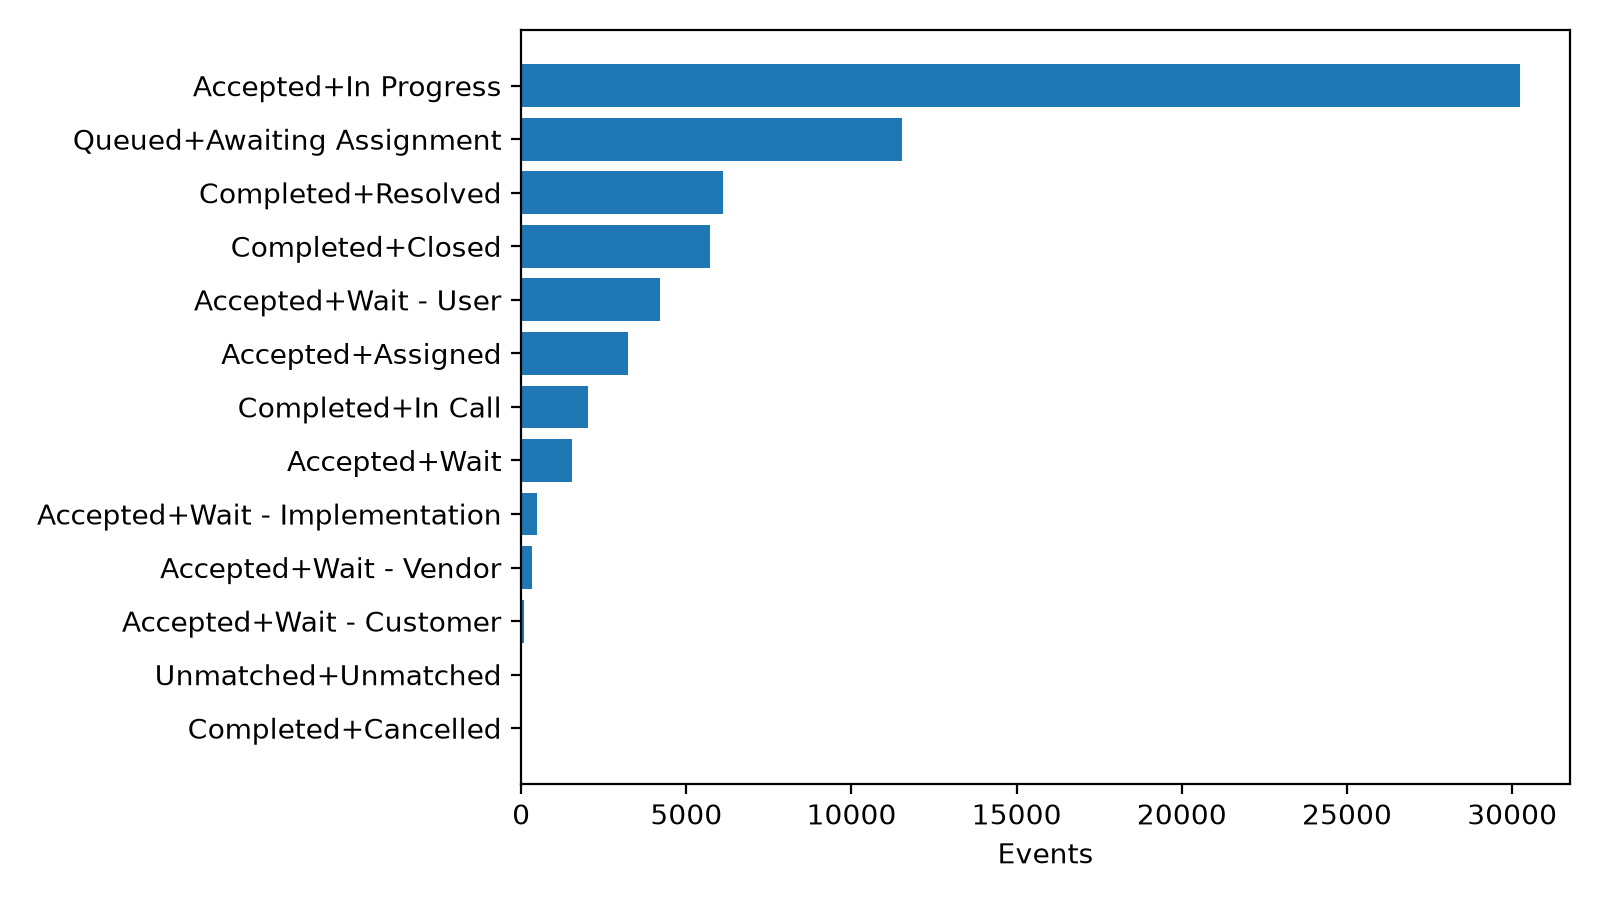
\includegraphics[width=\textwidth]{activity_frequency.png}
\caption{Event counts per activity in the incident log under the composite
labelling. \act{Accepted+In Progress} accounts for the plurality of all events.}
\label{fig:activity-frequency}
\end{figure}

\section{Process discovery}\label{sec:discovery}

\subsection{Algorithms}

Three algorithms are compared.

\begin{description}
  \item[Alpha miner] Infers ordering relations from directly-follows pairs and
        constructs a net from them. Simple and historically foundational, but it
        assumes the log is complete and noise-free, and it cannot represent
        short loops.
  \item[Heuristics miner] Weights the directly-follows relation by frequency and
        applies a dependency threshold, so infrequent behaviour is filtered out
        rather than modelled. Robust to noise.
  \item[Inductive miner] Recursively partitions the directly-follows graph and
        emits a process tree, which is converted to a net. Guarantees soundness
        and, at a noise threshold of zero, perfect fitness.
\end{description}

\subsection{Results}

\begin{table}[H]
\centering
\small
\begin{tabular}{llrrrrrr}
\toprule
Mode & Algorithm & Fitness & Precision & Gen. & Simpl. & Places & Trans. \\
\midrule
status & alpha & 0.119 & 0.400 & 0.734 & 1.000 & 2 & 4 \\
status & heuristics & 0.994 & 0.678 & 0.767 & 0.622 & 8 & 15 \\
status & inductive & 1.000 & 0.440 & 0.748 & 0.667 & 17 & 23 \\
status+substatus & alpha & 0.127 & 0.176 & 0.770 & 0.789 & 2 & 13 \\
status+substatus & heuristics & 0.948 & 0.387 & 0.634 & 0.471 & 27 & 69 \\
status+substatus & inductive & 1.000 & 0.234 & 0.783 & 0.634 & 57 & 78 \\
\bottomrule
\end{tabular}

\caption{Discovery on the full incident log; conformance computed on a sample of
cases. Both activity labellings are shown.}
\label{tab:discovery}
\end{table}

Three observations follow.

\paragraph{The fitness--precision trade-off is textbook.} The Inductive miner
attains perfect fitness in both labellings, as its construction guarantees, and
pays for it in precision: it buys replayability by being permissive, and it
produces by far the largest net. The Heuristics miner sacrifices a little
fitness for substantially better precision in a net a fraction of the size. If a
single model must be shown to a human, it is the Heuristics model.

\paragraph{The Alpha miner collapses, and theory predicts it.}
Its fitness falls below $0.15$ in both labellings and the net degenerates to two
places. This is not a defect in the implementation. Ninety percent of cases in
this log contain a length-one loop --- an activity immediately repeated --- and
the Alpha miner provably cannot represent such loops, because the ordering
relations it infers from a directly-follows pair $(a,a)$ are contradictory. The
result is a negative one worth reporting: it demonstrates the boundary of an
algorithm's applicability on a real log.

\paragraph{Finer labels cost precision.} Moving from four activities to thirteen
lowers precision for every algorithm and roughly triples model size, for the
reason given in Section~\ref{sec:mode}.

\begin{figure}[H]
\centering
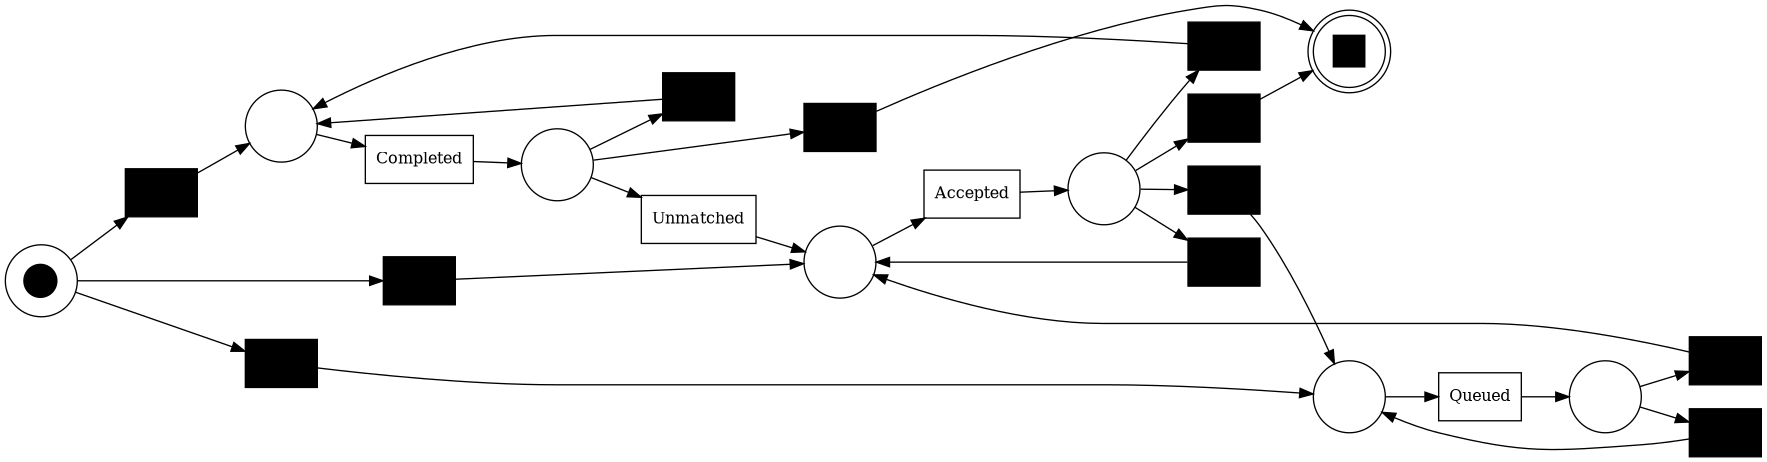
\includegraphics[width=0.85\textwidth]{petri_heuristics_status.png}
\caption{Heuristics miner, \act{Status} labelling. The best-balanced model of
those compared.}
\label{fig:petri-heuristics}
\end{figure}

\begin{figure}[H]
\centering
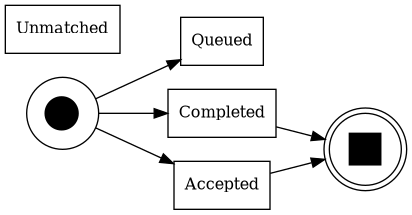
\includegraphics[width=0.6\textwidth]{petri_alpha_status.png}
\caption{Alpha miner, \act{Status} labelling. The degenerate structure is the
consequence of length-one loops, not of noise in the data.}
\label{fig:petri-alpha}
\end{figure}

\section{Performance analysis}\label{sec:performance}

\subsection{Method}

Waiting time is measured as the interval between an event and the next event of
the same case. The last event of a case has no successor and is therefore
excluded, rather than being recorded as zero; conflating the two would bias
every terminal activity downwards.

\begin{table}[H]
\centering
\small
\begin{tabular}{lrrrr}
\toprule
Activity & n & Mean (h) & Median (h) & Max (h) \\
\midrule
Completed+Closed & 143 & 143.31 & 95.28 & 736.50 \\
Accepted+Wait - Vendor & 313 & 131.63 & 28.15 & 1633.67 \\
Accepted+Wait - Implementation & 491 & 130.22 & 26.00 & 3500.55 \\
Accepted+Wait - Customer & 101 & 115.45 & 54.39 & 1488.93 \\
Completed+Resolved & 6,025 & 114.15 & 176.25 & 192.10 \\
Accepted+Wait - User & 4,214 & 109.97 & 26.36 & 5059.88 \\
Accepted+Wait & 1,533 & 97.99 & 3.45 & 4992.31 \\
Completed+In Call & 153 & 70.88 & 1.56 & 677.31 \\
Accepted+Assigned & 3,220 & 36.31 & 1.36 & 17334.07 \\
Queued+Awaiting Assignment & 11,544 & 26.16 & 0.59 & 6838.52 \\
Accepted+In Progress & 30,237 & 10.63 & 0.03 & 7896.28 \\
Unmatched+Unmatched & 5 & 0.19 & 0.07 & 0.61 \\
\bottomrule
\end{tabular}

\caption{Waiting time after each activity in the incident log. Both mean and
median are reported; see below for why either alone misleads.}
\label{tab:waiting}
\end{table}

\subsection{Mean and median diverge}

For \act{Accepted+In Progress} the median waiting time is on the order of
minutes while the mean is on the order of hours. The distribution is
heavy-tailed: work is normally picked up immediately and occasionally stalls for
a very long time. Reporting the mean alone would suggest a slow activity;
reporting the median alone would conceal the stalls. Both appear in
Table~\ref{tab:waiting} and in Figure~\ref{fig:waiting} for this reason.

\begin{figure}[H]
\centering
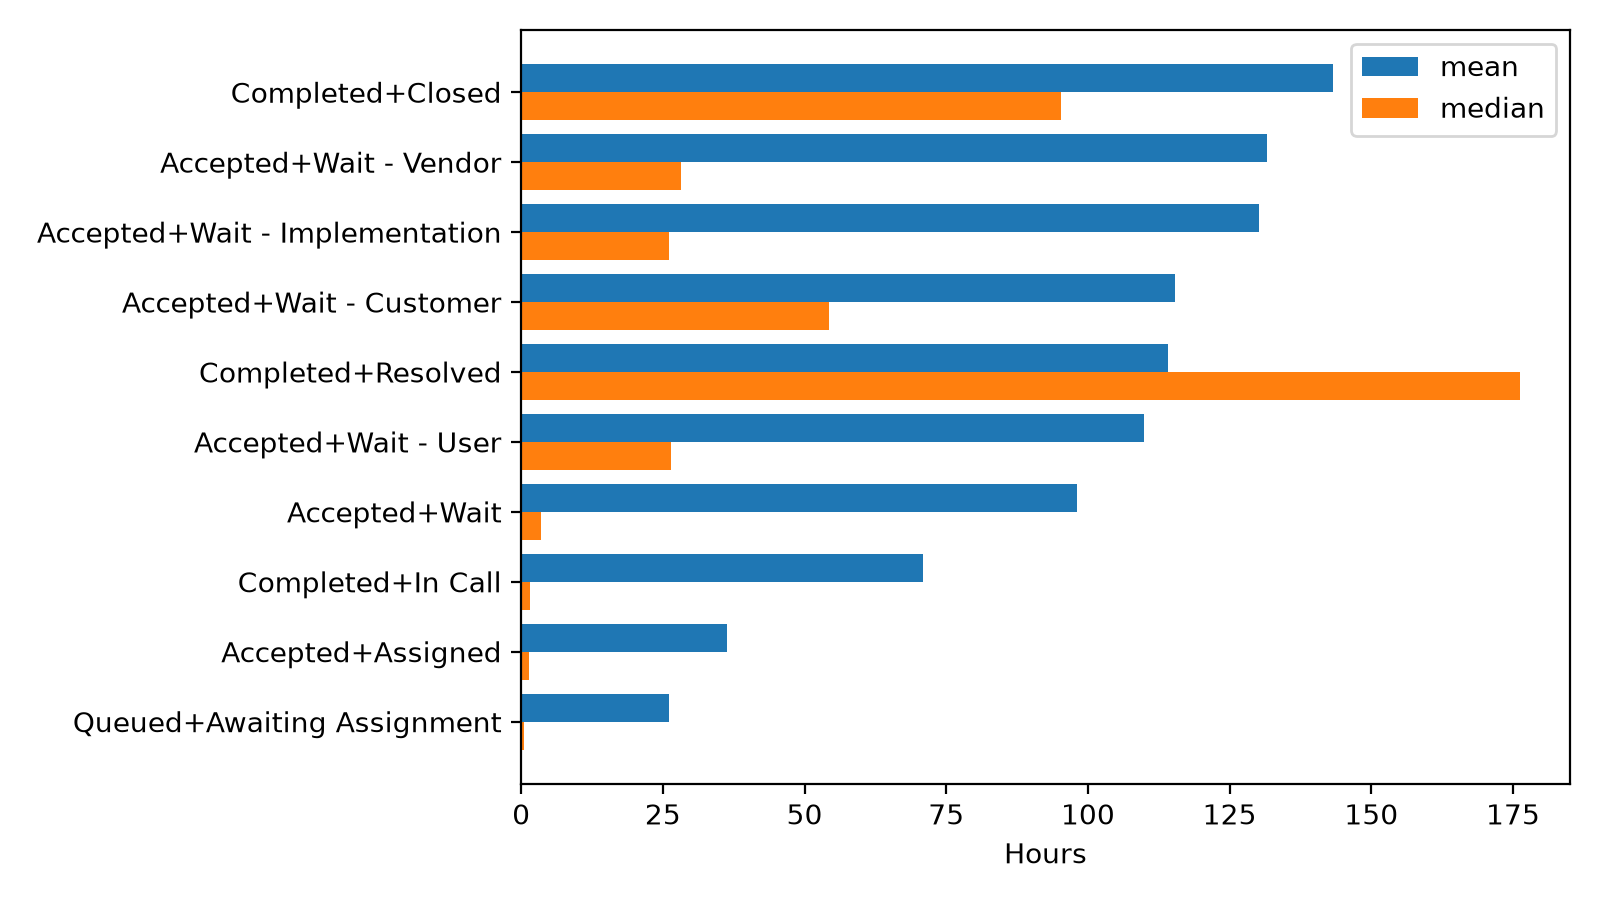
\includegraphics[width=\textwidth]{waiting_times.png}
\caption{Mean against median waiting time for the slowest activities. Where the
bars diverge sharply, the activity is usually fast and occasionally pathological.}
\label{fig:waiting}
\end{figure}

\subsection{Where the time goes}

The \act{Wait} states dominate mean waiting time: waiting on a vendor, on an
implementation, on a customer and on a user each average well over a hundred
hours. This is the expected shape for a support process whose delays are
external rather than internal, and it locates the improvement opportunity
outside the service desk itself.

One entry requires comment. \act{Completed+Closed} appears in
Table~\ref{tab:waiting} at all, which means a substantial number of closure
events were \emph{not} the last event of their case: work continued after the
incident was formally closed. Section~\ref{sec:verification} arrives at the same
conclusion by a completely different route.

\subsection{Duration and variability}

\begin{figure}[H]
\centering
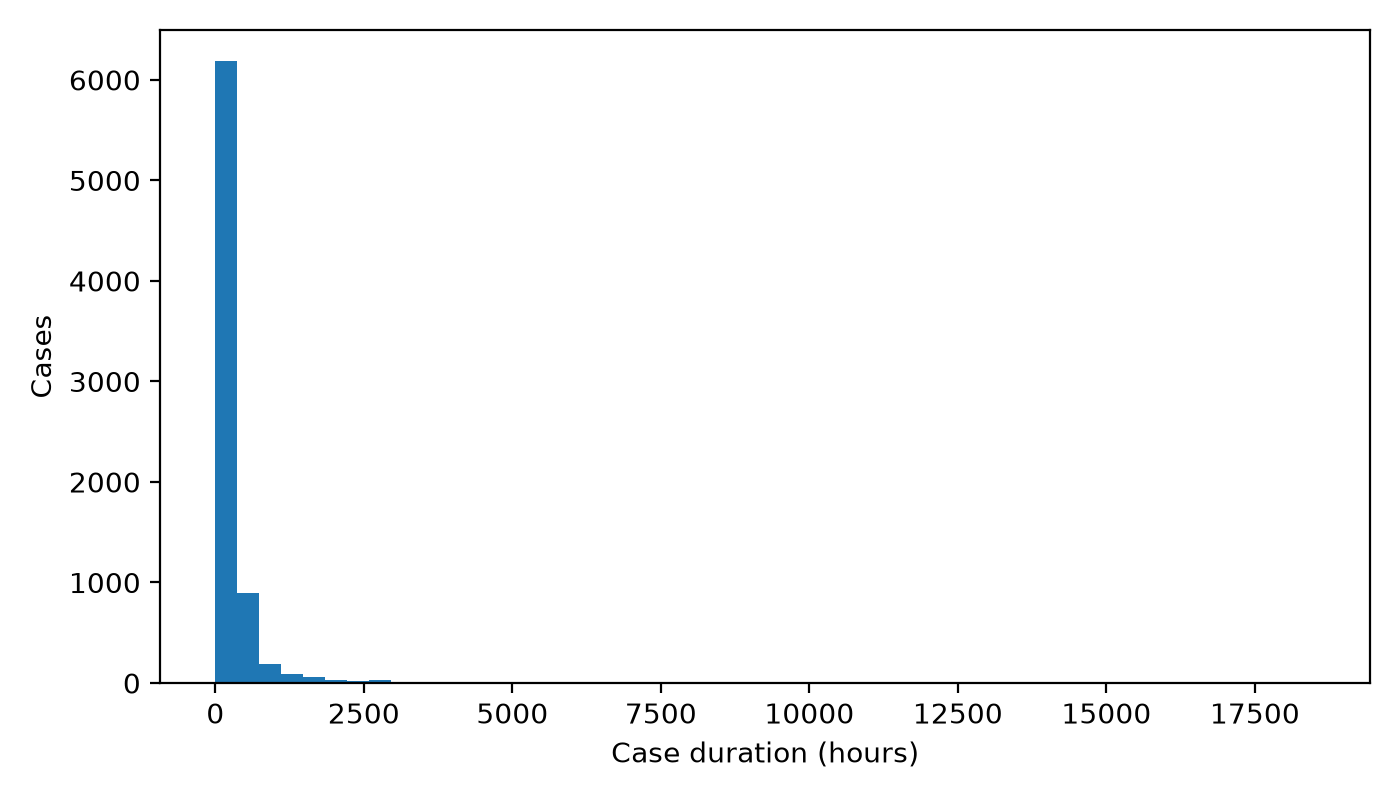
\includegraphics[width=0.8\textwidth]{duration_hist.png}
\caption{Distribution of case durations in the incident log.}
\label{fig:duration}
\end{figure}

\begin{figure}[H]
\centering
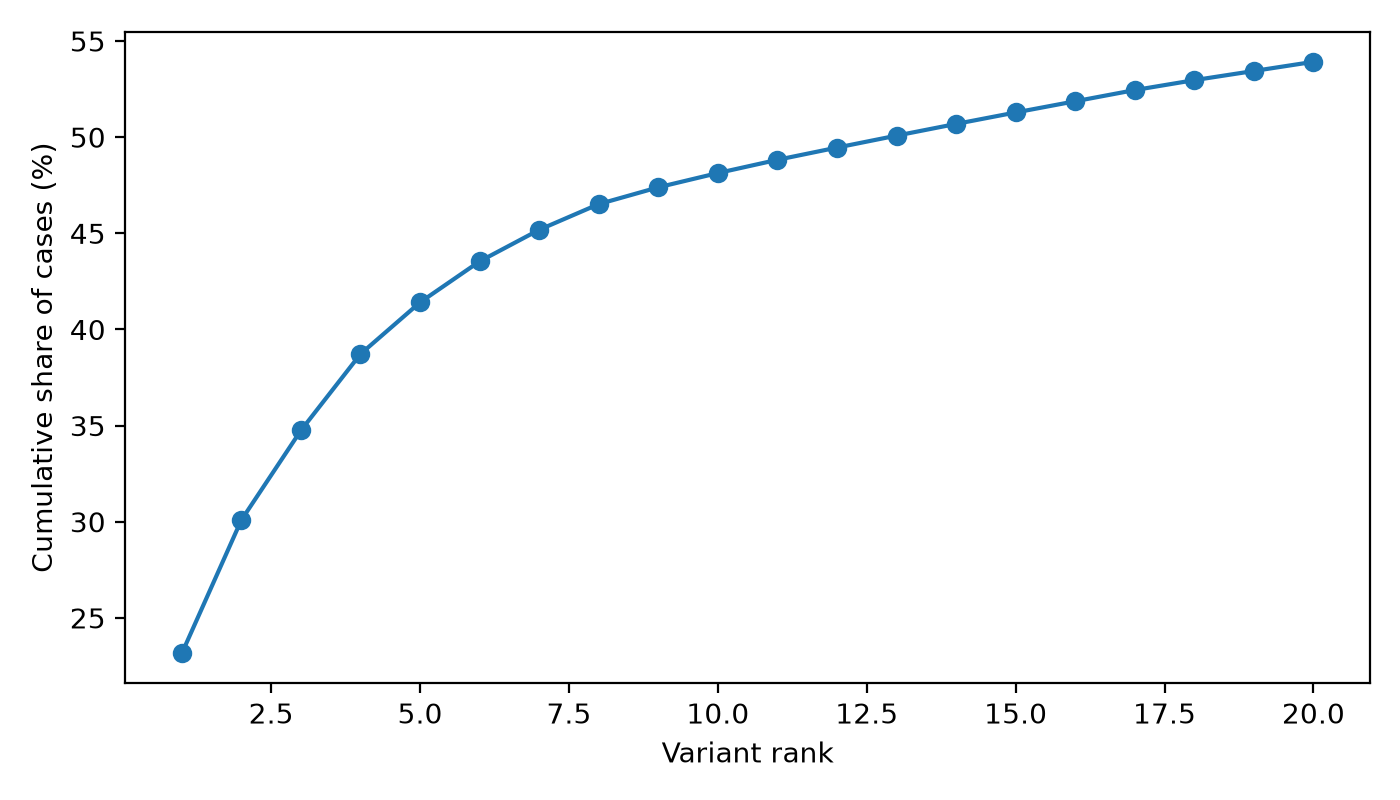
\includegraphics[width=0.8\textwidth]{variant_pareto.png}
\caption{Cumulative share of cases covered by the most frequent variants. The
curve flattens early: a large minority of cases follow paths that occur once.}
\label{fig:pareto}
\end{figure}

The process is only weakly standardised. Distinct variants number in the
thousands against seven and a half thousand cases, and the majority of variants
occur exactly once. Any model of this log with high precision would be
overfitted, which is the proper interpretation of the precision figures in
Table~\ref{tab:discovery}.

\section{Formal verification}\label{sec:verification}

\subsection{Specification}

Eight properties were specified in $\text{LTL}_f$ over the composite activity
alphabet, with activity labels mapped to proposition symbols
(\act{Accepted+In Progress} becomes \texttt{accepted\_in\_progress}). Each
property is evaluated independently against every case, and the satisfaction
ratio is the share of cases satisfying it. Cases that violate a property are
retained as counterexamples.

Six properties express expectations that ought to hold. Two express the
documented procedure, and are included precisely because they are expected to
fail; the size of the gap is the result.

\begin{table}[H]
\centering
\small
\begin{tabular}{lrrr}
\toprule
Property & Satisfied & Violated & Ratio \\
\midrule
Termination & 7,546 & 8 & 0.999 \\
Resolution & 7,545 & 9 & 0.999 \\
No work after closure & 7,435 & 119 & 0.984 \\
Queued work is picked up & 7,494 & 60 & 0.992 \\
Waiting on the user resumes & 7,550 & 4 & 0.999 \\
No unmatched events & 7,549 & 5 & 0.999 \\
Formal closure & 5,591 & 1,963 & 0.740 \\
Queueing precedes work & 1,168 & 6,386 & 0.155 \\
\bottomrule
\end{tabular}

\caption{Verification against all cases of the incident log.}
\label{tab:ltl}
\end{table}

\subsection{Interpretation}

\paragraph{The process terminates and resolves.} Termination, resolution, and
recovery from waiting on the user each hold for essentially every case. Whatever
else is wrong with this process, cases do not disappear into it.

\paragraph{Work continues after closure.} The property
\[
  \mathbf{G}\,(\texttt{completed\_closed} \rightarrow
  \neg\mathbf{F}\,\texttt{accepted\_in\_progress})
\]
fails for a small but non-trivial number of cases: an incident is formally
closed and then worked again. This corroborates, from the verification side, the
appearance of \act{Completed+Closed} in the waiting-time table of
Section~\ref{sec:performance}. Two independent methods agreeing is stronger
evidence than either alone.

\paragraph{Formal closure is not universal.} A quarter of incidents that are
worked never reach \act{Completed+Closed}; they are settled as
\act{Completed+In Call} instead. Whether this is a process defect or an
undocumented but legitimate resolution path is a question for the process owner.
The analysis establishes that the two routes coexist at scale.

\paragraph{Queueing does not precede work.} The documented procedure is that an
incident is queued for assignment and then taken up. Formally,
\[
  (\neg\,\texttt{accepted\_in\_progress}) \;\mathbf{U}\;
  \texttt{queued\_awaiting\_assignment}.
\]
This holds for a small minority of cases. In the large majority, work begins
without the incident ever having been queued. This is the ``push to front''
pattern for which the BPI 2013 dataset is known, and it is here established as a
formal property of the log rather than inferred from inspection of variants.

\subsection{A methodological result: strong next}\label{sec:strongx}

The no-work-after-closure property was first written in the form
\[
  \mathbf{G}\,(\texttt{completed\_closed} \rightarrow
  \mathbf{X}\,\mathbf{G}\,\neg\,\texttt{accepted\_in\_progress}),
\]
which is the natural formulation in infinite-trace LTL and reports a
satisfaction ratio of roughly one quarter --- an apparently severe process
failure. The figure is an artefact. As established in Section~\ref{sec:ltlf},
$\mathbf{X}$ is false at the final position of a finite trace, and the majority
of cases in this log \emph{end} with \act{Completed+Closed}. Every such case
falsifies the implication for reasons that have nothing to do with the process.

The $\mathbf{F}$-based formulation given above avoids the next operator entirely
and reports the true figure of roughly $98\%$. The two numbers differ by a
factor of nearly four, and only one of them is about Volvo IT.

The general lesson is that finite-trace semantics must be applied deliberately
when specifying properties of event logs, since a log is by construction a
collection of finite traces. Verification tooling that silently accepts an
infinite-trace formula will return a number, and the number will be wrong in a
direction that looks like a finding.

\section{Aggregate assessment}\label{sec:health}

To compare the three logs on one scale, a composite score aggregates four
normalised components: the share of cases reaching a completed state; the share
of events that are the first occurrence of their activity within their case;
one minus the variant ratio; and a throughput term derived from median case
duration against a fixed horizon.

\begin{table}[H]
\centering
\small
\begin{tabular}{lrlrrrr}
\toprule
Log & Score & Grade & Completion & Rework & Standardisation & Throughput \\
\midrule
closed\_problems & 65.9 & D & 1.000 & 0.655 & 0.780 & 0.000 \\
incidents & 74.4 & C & 0.999 & 0.481 & 0.698 & 0.748 \\
open\_problems & 70.0 & D & 0.435 & 0.746 & 0.778 & 0.942 \\
\bottomrule
\end{tabular}

\caption{Composite score and its components across the three logs. Higher is
better on every component.}
\label{tab:health}
\end{table}

The weighting and the throughput horizon are stipulated, not derived. The score
is therefore a comparison aid across logs and labellings and carries no absolute
meaning; this limitation is restated in Section~\ref{sec:threats}.

Read component-wise, one term dominates the incident log's result. Completion is
near perfect and variability is moderate, but fewer than half of all events are
first occurrences of their activity. \textbf{Over half of all recorded work in
the incident process is repetition.} This is the single largest lever available
and it is consistent with the picture from every other section: heavy looping,
work resumed after closure, and thousands of one-off variants.

\section{Implementation}\label{sec:architecture}

The analysis is implemented as a Python package organised in four layers.

\begin{description}
  \item[Loading] Parses either distributed form of the dataset, derives the
        activity label according to the selected mode, and retains every source
        attribute. Reducing events to the three XES-standard columns, as is
        common, would discard the organisational data on which any extension of
        this work depends.
  \item[Mining] Discovery, conformance and algorithm comparison.
  \item[Verification] Activity-to-proposition encoding, $\text{LTL}_f$
        evaluation per trace, and counterexample extraction.
  \item[Analysis] Waiting times, durations, variants, statistical anomalies, a
        first-order Markov transition model and the composite score.
\end{description}

Every analysis function is stateless: it takes a loaded log and returns a value,
holding no module-level state. A browser-based dashboard presents the layers
interactively, holding the loaded log in per-session state, and a report
generator produces documents of this kind from the same functions. The
statelessness is what makes the analysis testable without a web server; the
suite comprises well over a hundred tests, including regression tests that pin
the measured figures reported here.

All tables and figures in this report are generated from the analysis code. No
measured value has been transcribed by hand.

\section{Conclusions}\label{sec:conclusions}

\subsection{Findings}

\begin{enumerate}
  \item \textbf{Rework dominates.} Fewer than half of the events in the incident
        log are the first occurrence of their activity within the case. The
        majority of recorded work is repetition, and this is the principal
        driver of the aggregate score.
  \item \textbf{The documented procedure is not the executed procedure.}
        Queueing before work holds for a small minority of cases; the ``push to
        front'' pattern is dominant. This was established by formal verification
        over every case, not by sampling or inspection.
  \item \textbf{The Alpha miner is inapplicable to this log.} Its failure is
        predicted by the prevalence of length-one loops and constitutes a
        demonstration of a known theoretical boundary rather than an empirical
        surprise.
\end{enumerate}

\subsection{Threats to validity}\label{sec:threats}

\begin{itemize}
  \item Conformance metrics are computed on a sample of cases rather than the
        full log, because alignment-based computation does not terminate in
        reasonable time at full scale. Sampling is deterministic but not random.
  \item Token-based replay, used for the headline figures, is an approximation
        and is known to be optimistic on unsound nets. Alignment-based
        computation is implemented and available, and agrees on the sample.
  \item The composite score's weights and horizon are stipulated. Component
        values are meaningful; the aggregate is meaningful only comparatively.
  \item \act{Unmatched+Unmatched} is an artefact of the VINST export rather than
        a process step. It is retained rather than filtered, so that its
        prevalence is visible, but it should not be read as work.
  \item Findings concern what the system recorded. Work performed but not
        recorded is invisible to every method used here, and a process with poor
        recording discipline will appear to have more rework than it has.
\end{itemize}

\subsection{Further work}

The loader retains the organisational attributes that this analysis does not yet
use. The natural continuations are handover-of-work analysis across the support
lines, quantification of the push-to-front pattern by organisation rather than
by trace shape, and comparison of the incident and problem processes as distinct
but interacting systems. Each is supported by the data already loaded.

\end{document}
